\section{Zielsetzung}
In diesem Versuch werden Reflexion, Brechung und Beugung auf ihre Gesetzmäßigkeiten überprüft.

\section{Theoretische Grundlagen}
Licht besteht aus elektromagnetischer Strahlung.
Das für das menschliche Auge sichtbare Lichtspektrum befindet sich im Wellenlängenbereich von 380 nm bis 780 nm, 
auf den sich in diesem Versuch beschränkt wird.
Im folgenden werden verschiedene Phänomene mithilfe der Strahlen- und Wellenoptik näher erläutert.

\subsection{Reflexion und Brechung}
In der Strahlenoptik wird das Licht auf die Wellennormale, 
die senkrecht auf der Wellenfront steht und als Lichtstrahl bezeichnet wird, beschränkt.
Mithilfe der Strahlenoptik können im folgenden zwei Vorgänge genauer betrachtet werden:

\begin{enumerate}
\item Reflexion

Trifft ein Lichtstrahl auf eine Grenzfläche, so wird dieser zurückgeworfen, anstatt im Medium weiter zu propagieren.
Dabei gilt das Reflexionsgesetz

\begin{equation}
\alpha_1 = \alpha_2,
\label{eqn:refl}
\end{equation}

das besagt, dass der Einfallswinkel gleich dem Ausfallswinkel ist.

\item Brechung

Fällt ein Lichtstrahl auf eine Grenzfläche eines anderen Mediums mit Brechungsindex n und breitet sich in diesem aus,
ändert sich die Ausbreitungsgeschwindigkeit und der Lichtstrahl ändert seine Richtung.
Der Lichtstrahl wird gemäß des Gesetzes von Snellius gebrochen, nach dem gilt:

\begin{equation}
\frac{sin \, \alpha}{sin \, \beta} = \frac{n_2}{n_1} = \frac{v_1}{v_2} 
\label{eqn:snel}
\end{equation}

Dabei sind $n_1$ und $n_2$ die Brechungsindizes des ersten und zweiten Mediums und $v_1$ und $v_2$ die jeweiligen Ausbreitungsgeschwindigkeiten.
Das Material mit der größeren Ausbreitungsgeschwindigkeit wird als optisch dichter und das mit der kleineren als optisch dünner bezeichnet.
Beim Übergang von einem optisch dünneren zu einem dichten Medium wird der Lichtstrahl zum Lot hin gebrochen.
Da in diesem Versuch für den Brechungsindex $n_1\approx$1 mit Luft als optisch dünnerem Medium gilt, 
kann das Brechungsgesetz zu

\begin{equation}
    \frac{sin \, \alpha}{sin \, \beta} = n
    \label{eqn:snell}
\end{equation}

vereinfacht werden.

\end{enumerate}

\noindent
In der Realität finden zumeist Reflexion und Brechung gleichzeitig statt.
Der Lichtstrahl teilt sich in einen Teil mit der Intensität $R$ der reflektiert, und einen Teil mit der Intensität $T$ der transmittiert wird auf.
Dabei gilt stets $R + T = 1$.
Das Prinzip der Rexflexion und Brechung ist in Abbildung \ref{fig:rt} dargestellt.

\begin{figure}
    \centering
       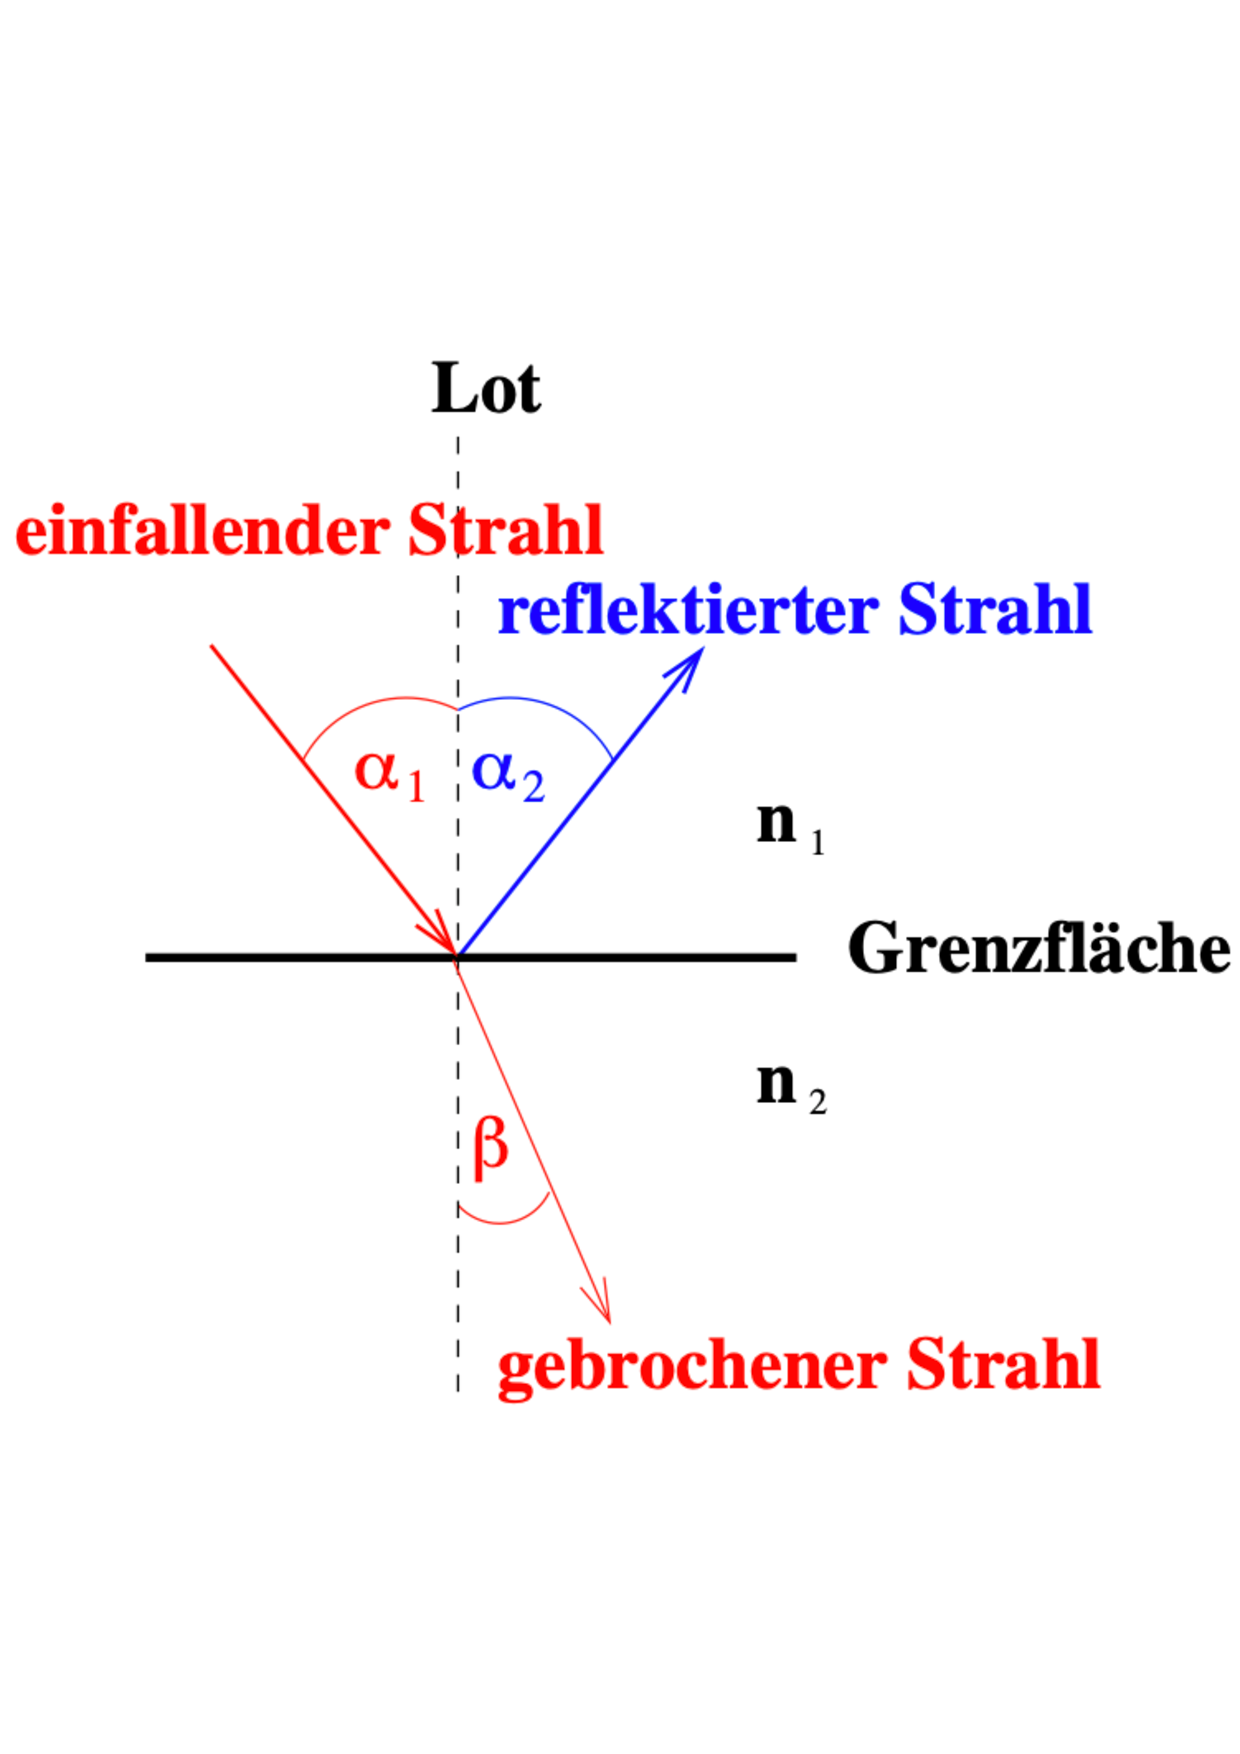
\includegraphics[height=5cm]{rt.pdf}
       \caption{Reflexion und Brechung eines Lichtstrahls (Quelle: \cite{V400}).}
       \label{fig:rt}
\end{figure}

\noindent
\textbf{Planparallele Platten}

\noindent
Mit der Reflexion und Brechung kann nun der Strahlversatz an einer planparallelen Platte aus Abbildung \ref{fig:plan} hergeleitet werden.

\begin{figure}
    \centering
       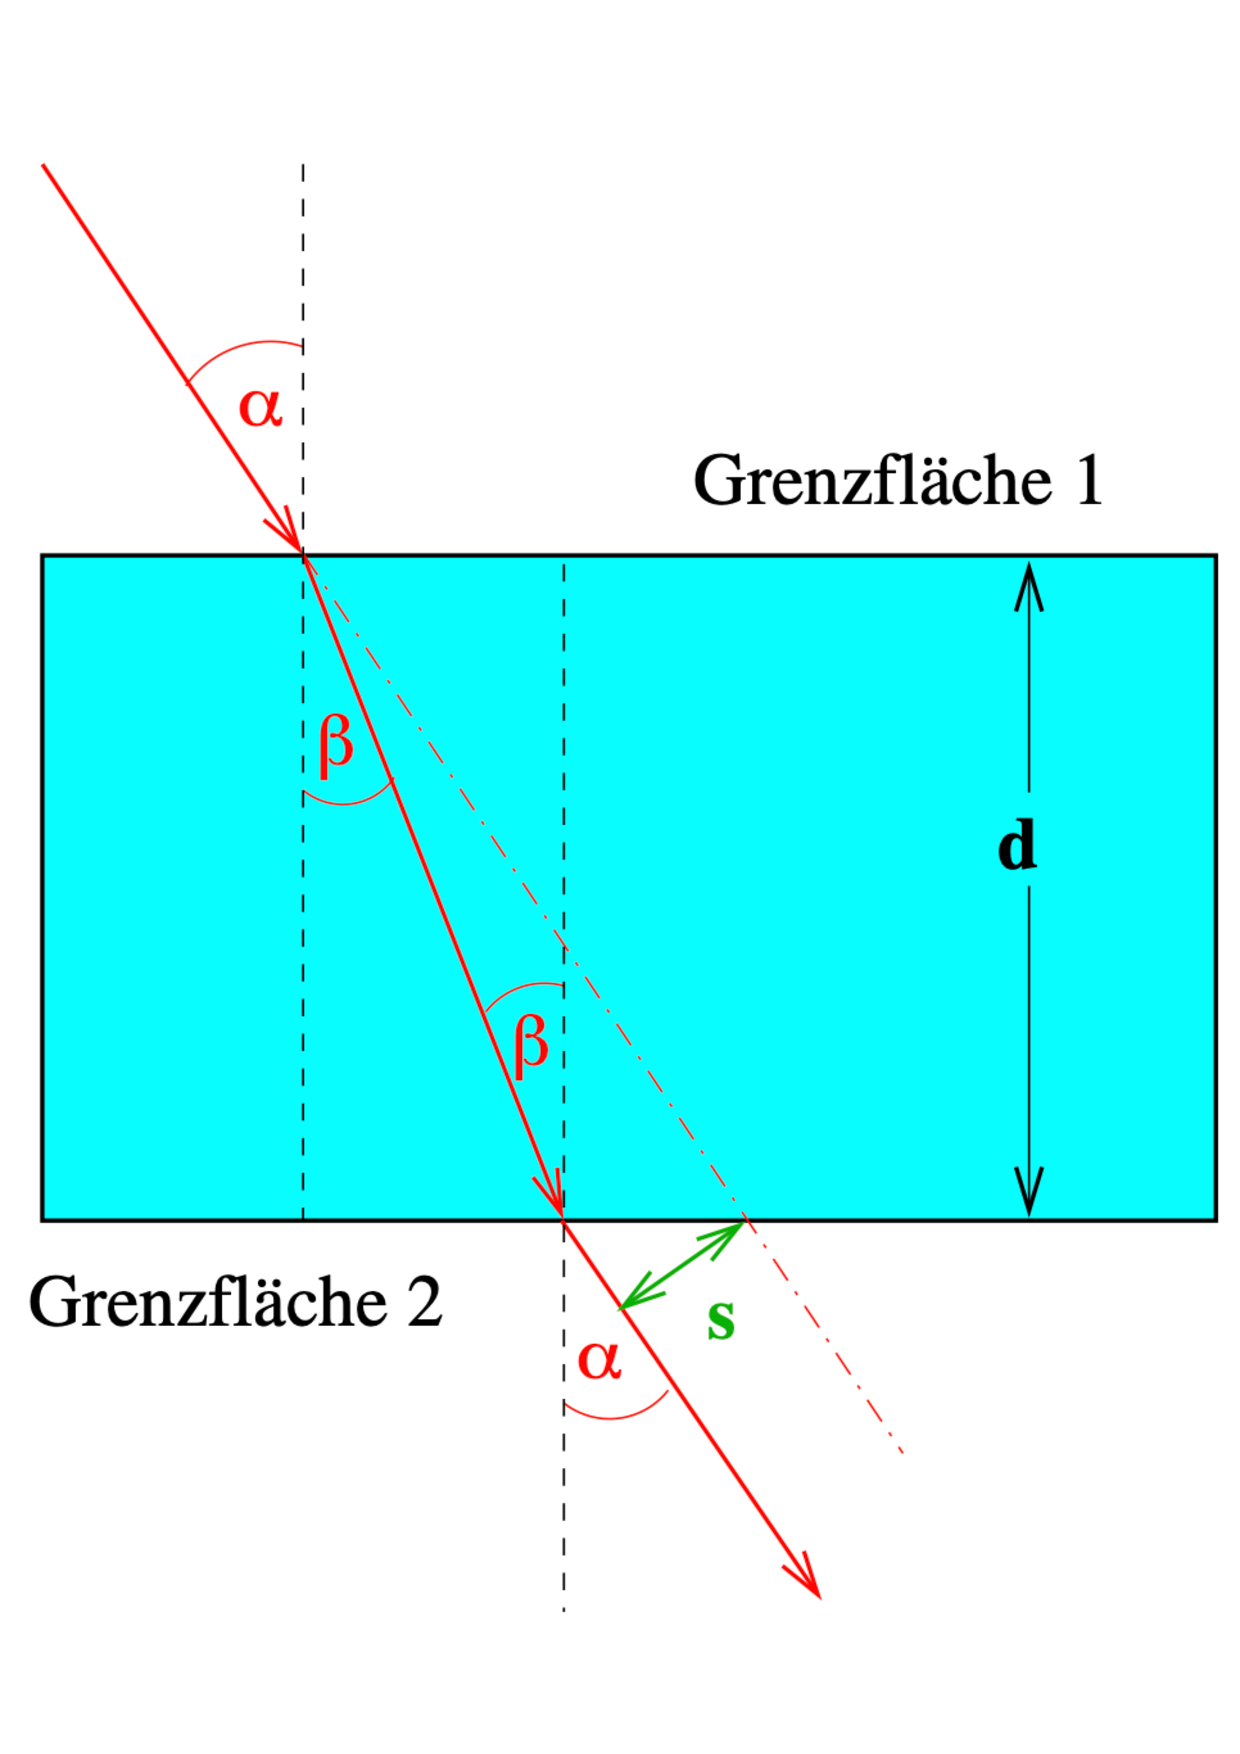
\includegraphics[height=5cm]{plan.pdf}
       \caption{Strahlversatz an einer planparallelen Platte (Quelle: \cite{V400}).}
       \label{fig:plan}
\end{figure}

\noindent
Der auf die planparallele Platte treffende Lichtstrahl wird am optisch dichteren Medium an der Grenzfläche zum Teil reflektiert und zum Lot gebrochen.
Da der gebrochene Lichtstrahl an der zweiten Grenzfläche erneut gebrochen wird, diesmal jedoch zur Grenzfläche hin,
erfährt dieser keine Richtungsänderung sondern nur einen Strahlversatz $s$, der durch 

\begin{equation}
s = d \, \frac{sin\, (\alpha-\beta)}{cos\,\beta}
\label{eqn:s}
\end{equation}

\noindent
beschrieben werden kann.

\newpage
\noindent
\textbf{Prisma}

\noindent
Das optische Prisma ist in Abbildung \ref{fig:prism} Dargestellt.

\begin{figure}
    \centering
       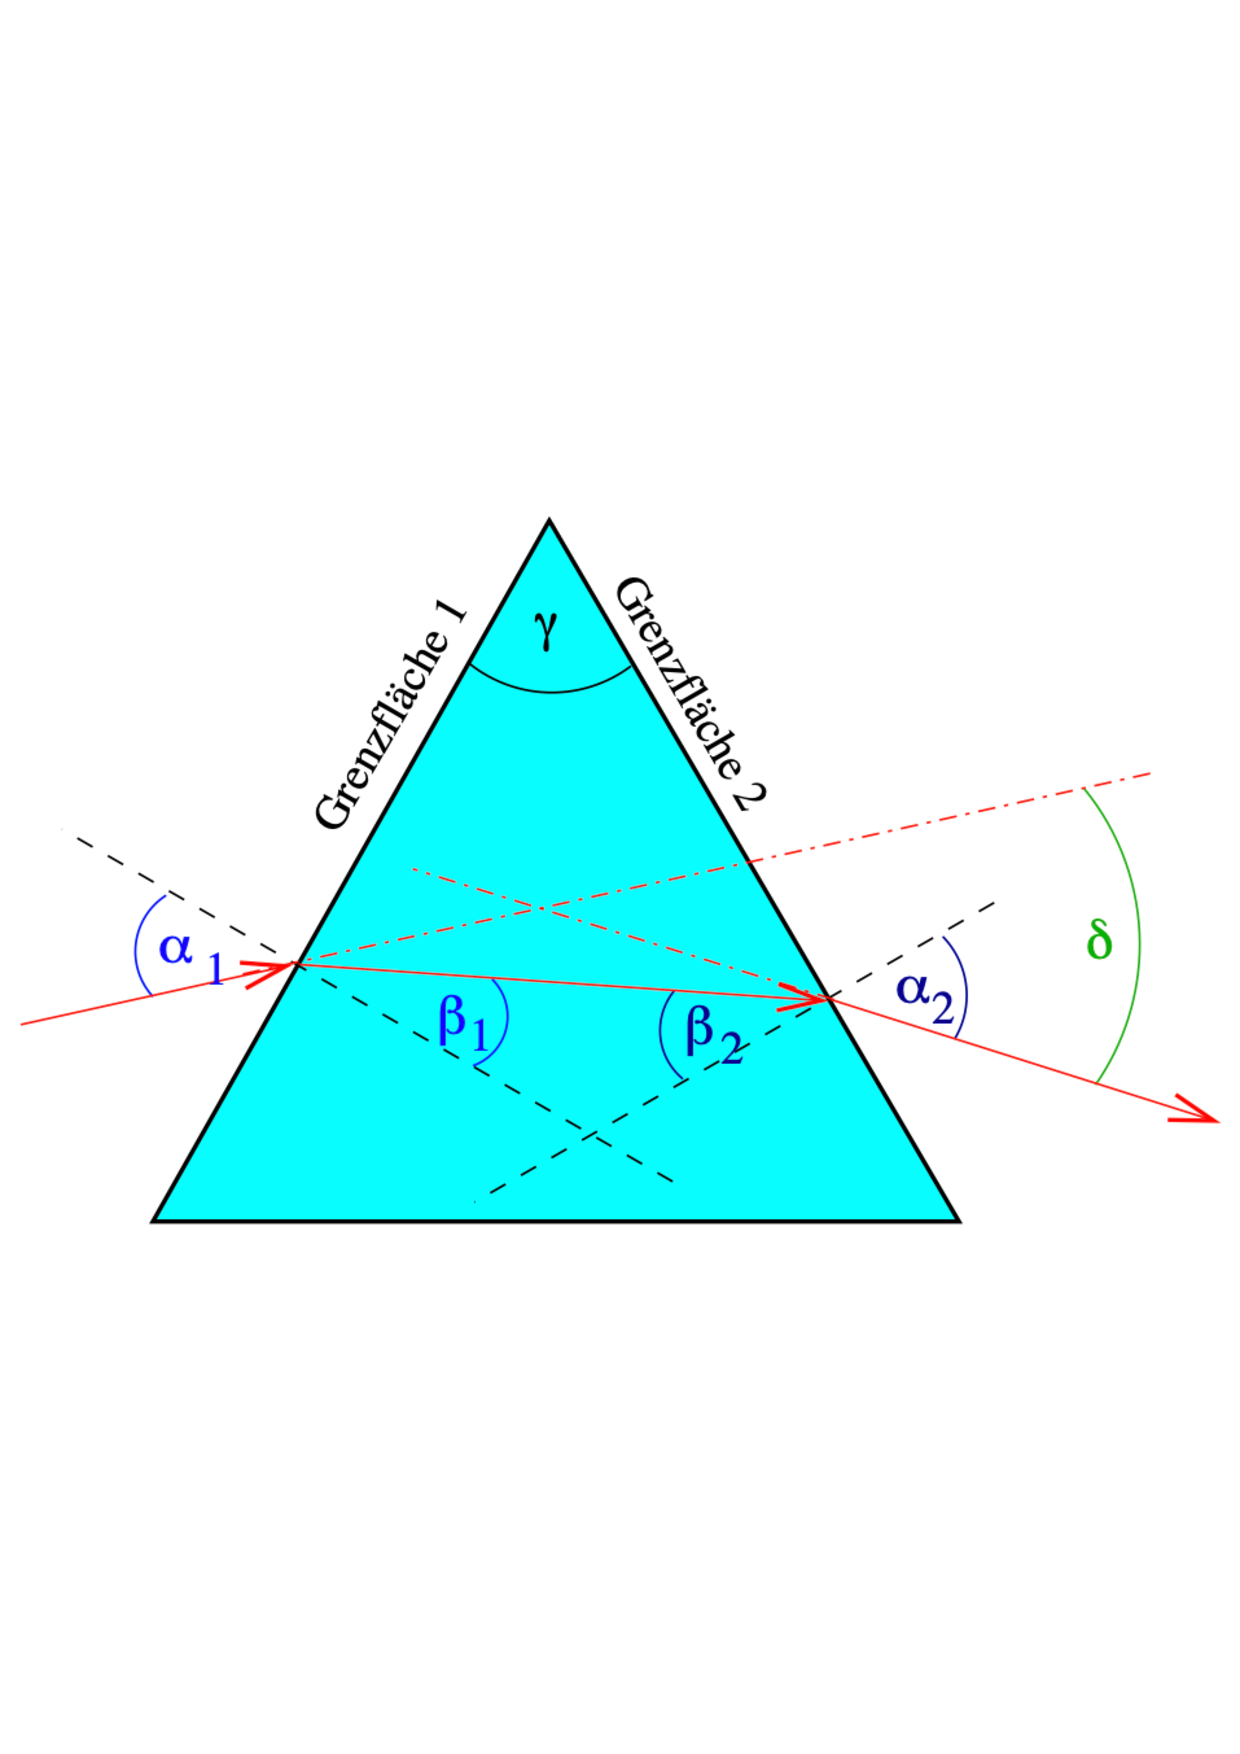
\includegraphics[height=5cm]{prism.pdf}
       \caption{Brechung am optischen Prisma (Quelle: \cite{V400}).}
       \label{fig:prism}
\end{figure}

\noindent
Die brechenden Kanten des Prismas durch die der Lichtstrahl ein- und austritt stehen nicht parallel zueinander und begrenzen den brechenden Winkel $\gamma$.
Die Ablenkung 

\begin{equation}
    \delta = ( \alpha_1 + \alpha_2) - (\beta_1 + \beta_2)
\end{equation}

\noindent
die durch zweifache Brechung an den Grenzflächen entsteht, 
ist abhängig von der Wellenlänge des Lichtes. 
Diese Abhängigkeit wird als Dispersion bezeichnet.

\subsection{Beugung}
Unter der Beugung versteht man die Ausbreitung des Lichtes im Schattenraum nachdem es auf ein Hindernis getroffen ist.
Um das Phänomen der Beugung erklären zu können, 
wird sich nun auf die Wellenoptik bezogen.
Charakteristische Welleneigenschaften sind die Wellenlänge $\lambda$ 
und die Ausbreitungsgeschwindigkeit $v$.
Bei der Überlagerung von Wellen addieren sich die Intensitäten in jedem Punkt zu einer resultierenden Intensitätsverteilung.
Wenn die einzelnen Wellenzüge dieselbe Frequenz und eine feste Phasenbeziehung haben,
entsteht ein Interferenzbild.
Abhängig von der Phasenbeziehung kommt es zur konstruktieven (verstärkenden) oder zur destruktiven (abschwächenden) Interferenz.
Gelangt Licht durch ein Gitter, kommt es zur Beugung wenn die Spaltbreite $d$ klein im Vergleich zur Wellenlänge ist.
Für die Intensitätsmaxima des Interferenzmusters gilt die Beziehung

\begin{equation}
d \, sin \, \alpha = k\, \lambda.
\label{eqn:beug}
\end{equation}

\noindent
Dabei ist $d$ die Gitterkonstante, $\alpha$ der Winkel relativ zur gradlinigen Ausbreitungsrichtung und k die Ordnung des Maximums.

